%==============================================================================
% @author Clinton Freeman
% @date 12/18/2013
%==============================================================================

\documentclass[oneside]{memoir}   

\usepackage{rc_style} 

\begin{document} 

%==============================================================================
% Cover page
%==============================================================================
   
\frontmatter

%\pagecolor{answerColor}
%\color{white}

\pagenumbering{gobble}
\thispagestyle{empty}     

%\begin{mdframed}[style=answer]  
\noindent{\fontsize{48pt}{64pt}\myfont\selectfont Rational\textbf{CAD} 0.1}
    
\vspace{1.5em}   

\noindent{\fontsize{24pt}{48pt}\myfont\selectfont User Manual}
%\end{mdframed}   
%\vspace{10em}  
\par\vspace*{\fill}

%\noindent\hfill{\fontsize{16pt}{24pt}\selectfont by CLINTON FREEMAN}  

\clearpage
 
%\pagecolor{white}   
%\color{black}

%\newpage\null\thispagestyle{empty}\newpage  

%==============================================================================
% Table of Contents 
%==============================================================================

\pagenumbering{roman}

\begingroup
\hypersetup{linkcolor=black}
\tableofcontents*
\endgroup   
 
\clearpage

%==============================================================================
% Preface
%==============================================================================

% \chapter{Preface}  
% 
% I am writing this book because I have yet to find a single source that clearly
% outlines what is to be done about geometric nonrobustness from both a
% theoretical and practical point of view.
% 
% \vspace{2em}
% \hfill\textbf{Clinton Freeman}
% 
% \hfill\textit{Chapel Hill, North Carolina}
% 
% \hfill January 2014

%==============================================================================
% Introduction
%==============================================================================

\mainmatter   
\pagenumbering{arabic}
     
\chapterstyle{freeman}

\chapter{Introduction}         
 
% \chapterprecishere{``Begin at the beginning,� the King said gravely, ``and go on
%  till you come to the end: then stop."\par\raggedleft--- \textup{Lewis Carroll}, Alice in Wonderland}

%\epigraph{``Begin at the beginning," the King said gravely, ``and go on till
% you come to the end: then stop."}{--- \textup{Lewis Carroll}, Alice in Wonderland}
 
RationalCAD allows users to create robust, error-free geometric models from
convex polytopes. This document describes what RationalCAD is, how it differs
from other editors, and how to use its powerful features to build complex 3D
models. It is written for RationalCAD version 0.1 for Windows x64.

\section{Interface Overview}
 
\begin{figure}[h!]
  \centering
    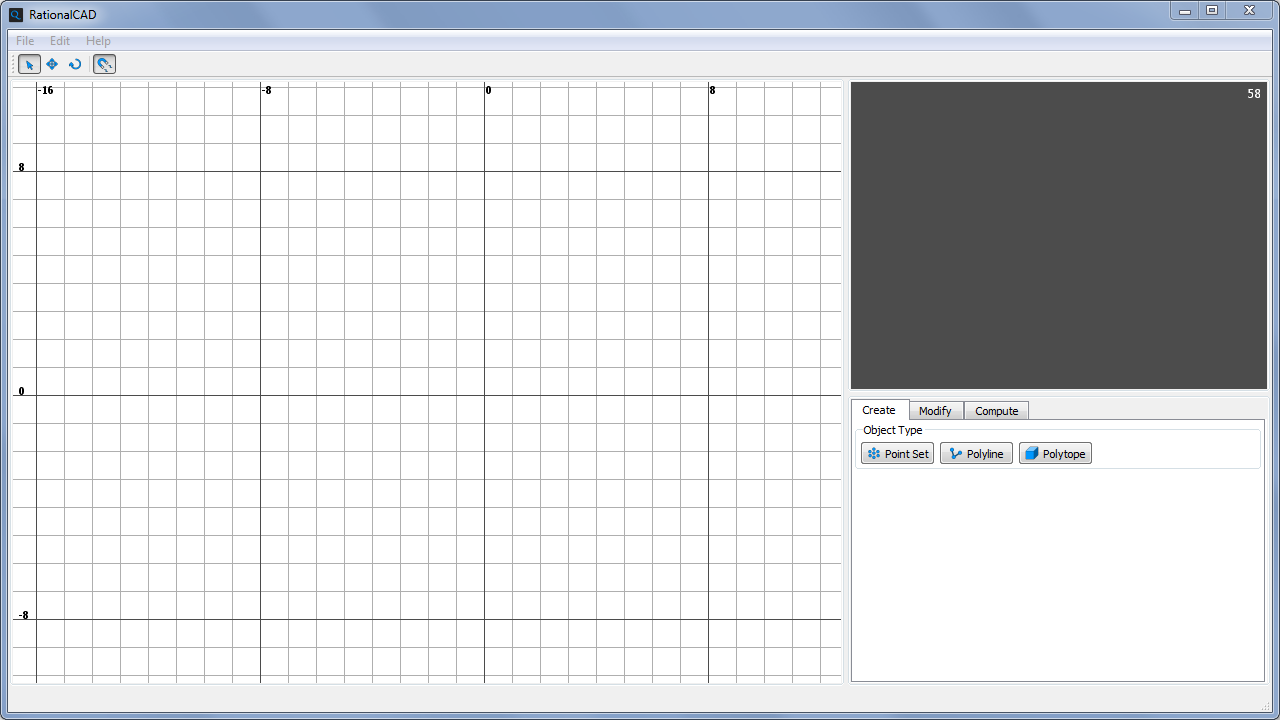
\includegraphics[width=0.9\textwidth]{images/interface-overview}
\end{figure}

The Graphical User Interface (GUI) comprises 7 components: the menubar, the
toolbar, the orthographic widget, the perspective widget, the interactive panel,
the statusbar, and the console.

% ![GUI Overview](http://cs.unc.edu/~freeman/DDAD/media/gui-overview.png)
\subsection{Menubar} 

The menubar comprises 3 high-level menus: File, Edit, and Help. It exists
primarily as a scaffold for future functionality.

\subsubsection{File} 

The File menu is currently empty but
\href{https://github.com/unc-compgeom/DDAD/issues/6}{issue $\triangle$ 6} 
specifies saving and loading of files. To do this, we need a mechanism for
serializing and deserializing the scene, which is a major undertaking.
 
\subsubsection{Edit}
 
The Edit menu contains one element, Preferences (there are issues to add
duplicating and copy/paste.) Clicking Preferences will open a dialog which is
split into 3 major panels. On the left is a list of subsections. The list
currently contains only Grid Settings. On the right is a detailed view of the
selected subsection. This detail view is parameterized by the list on the left.
Finally, the bottom contains 4 buttons: Default, Cancel, Apply, and Ok. The most
interesting of these is Default, which requires the application to somehow
define defaults. Settings \& Defaults bring up the notion of a configuration
file (e.g. .ini). While currently there are not many settings, the dialog sets
forth a framework into which developers can add new configurations settings.
    
\subsubsection{Help} 

The Help menu contains two simple elements. The first is a link to the user
manual (the wiki). The second is an About dialog that provides information about
the program version and a link to the project webpage.

\subsection{Toolbar} 

The toolbar comprises 4 elements: 3 buttons to control input mode (Select,
Translate, and Rotate), and 1 button to toggle snapping to grid. The three input
mode buttons are mutually exclusive with one another and with the creation
buttons in the interactive panel. The select mode is initially activated and
allows the user to pick one object at a time via left-clicking in the
orthographic and perspective views.
\href{https://github.com/unc-compgeom/DDAD/issues/8}{Issue $\triangle$ 8}
specifies multiple-object selection,
\href{https://github.com/unc-compgeom/DDAD/issues/9}{issue $\triangle$ 9}
specifies the rotation mode, and
\href{https://github.com/unc-compgeom/DDAD/issues/10}{issue $\triangle$ 10}
specifies the translation mode.

\subsection{Orthographic Widget} 

The orthographic widget allows users to precisely create and manipulate objects
against the backdrop of an integer grid. The integer grid has minor and major
grid lines. Minor lines are drawn in a lighter color. Major lines occur after a
certain number of minor lines - the default is 8.

Users are able to zoom in and out and pan around the grid. As the user zooms
out, the grid adapts so that the lines are not drawn too close together. At the
highest zoom level, minor lines are drawn 1 unit apart. After the user zooms out
a ways, the grid adapts to draw minor lines 8 units apart. After more zooming,
the grid adapts to draw minor lines 64 units apart, and so on.

\subsubsection{Current Limitations}

The orthographic widget only draws a top-down (XY plane) view.

\subsubsection{Controls}

\noindent\begin{tabularx}{\textwidth}{lX}
\toprule 
Action & Command \\  
\midrule
Pan & Click and hold middle mouse button, then drag \\

Zoom & Scroll mouse wheel \\

Activate current tool & Left mouse click \\

Open context menu & Right mouse click \\
\bottomrule
\end{tabularx}  

\subsection{Perspective Widget} 

The perspective widget allows the user to control a 3D perspective camera that
renders the current scene. It provides a small frames per second (FPS)
counter in the top right corner. Users may change the camera's orientation and
move in several directions, outlined below. The perspective widget may be
activated and deactivated to enable or disable camera movement. Once activated,
the user is shown a small crosshairs symbol indicating the current camera view
direction.

\subsubsection{Controls}

\noindent\begin{tabularx}{\textwidth}{lX}
\toprule 
Action & Command \\  
\midrule
Activate/Deactivate & Right mouse click \\

Change camera orientation & Move mouse \\

Move forward & W \\

Move backward & S \\

Strafe left & A \\

Strafe right & D \\

Move up & Spacebar \\

Move down & C \\
\bottomrule
\end{tabularx}  

\subsection{Interactive Panel} 

The interactive panel comprises three tabs: Create, Modify, and Compute.

The create tab is open by default. It initially has only a gallery of geometric
objects. The buttons in the gallery are mutually exclusive with one another and
with the input mode buttons in the toolbar. Once the user selects one of the
geometric objects, an additional ``Creation Method'' panel will appear with
additional options. The options are parameterized by the selected object type;
often these methods will overlap (e.g. clicking inside the orthographic view to
create a point set or polyline), but may be unique (e.g. a polytope may have a
user-defined length, width, and height). Each method will be listed in a
dropdown menu at the top of the panel. As the user changes between methods,
method-specific controls will appear below the dropdown. For example, when
``Click'' is selected, explanatory text appears; if you change the selection to
``File,'' then the explanatory text will be replaced with a file chooser and
``Generate'' button.

The modify tab is meant to let the user choose the \emph{selection granularity},
or the level at which operations are applied. For example, a polytope is
composed of vertices, edges, and faces. Each of these, along with the whole
polytope, are selectable levels of granularity. When ``edges'' is selected,
picking operations will choose from only the object's edges, when ``vertices''
is selected, picking operations will choose from only the object's vertices, and
so on. Most of this functionality is not yet implemented, but is specified in
\href{https://github.com/unc-compgeom/DDAD/issues/7}{issue $\triangle$ 7}.

The compute tab is composed of the name of the selected object and a drop down
menu of applicable algorithms. The dropdown of algorithms follows the same logic
as the creation method dropdown, meaning that as you change your selection
relevant parameters will appear below. Once the user is with the algorithm
selection and any parameters, they would like to execute the algorithm. For
this, we provide a set of media controls. In particular, they may click the
``Run'' button which will begin algorithm execution. Once the algorithm is
running, editing controls will be disabled.

\subsection{Statusbar.} The statusbar provides a way of sending messages to the
user, depending on application context. For example, when the user is creating a
polyline, the application cycles through 2 different states. First, the user
needs to click in the orthographic view to position the initial vertex, so we
might simply display: ``Left-click in the orthographic view to place first
vertex.'' Second, the user can either place additional vertices in the same
fashion, or terminate the polyline by right-clicking; the status bar should be
updated to reflect the user's options: ``Left-click again to add more vertices,
or right-click to terminate polyline.'' Finally, after the user right-clicks to
terminate, we transition back to creating a new polyline, so the message should
update as well.

The main window defines a slot for updating the statusbar message (\texttt{void
onUpdateStatusBarMsg(const QString\& status)}). To trigger the handler from
another QObject, you must ensure that the instance is connected to the main
window, then emit an appropriate signal. For more information, see Qt's
documentation on
\href{http://qt-project.org/doc/qt-4.8/signalsandslots.html}{signals and slots} and
\href{http://qt-project.org/doc/qt-4.8/qstatusbar.html}{QStatusBar}.

\subsection{Console.}

The console is designed to provide non-developers with useful information in
case they experience unexpected (but non-terminal) behavior. By logging to the
console, developers can ask these users to inspect the console to understand the
application behavior. The console is not meant as a replacement of the IDE
console. By default, the console is hidden from view, but may be expanded at any
time.

\chapter{Geometric Objects}

\section{Point Set}

\subsection{Creation Methods}

\subsubsection{Click}

Allows the user to left-click in the orthographic widget to place individual
points in the set, then right-click to finish creation.

\subsubsection{File}

Allows the user to read in a simple text file that lists the XYZ coordinate
tuples of the point set.

\subsection{Modifications}

\subsection{Computations}

\subsubsection{Terrain Mesh}

This computes a terrain mesh from the point set using Delaunay triangulation.

%\subsubsection{Convex Hull}

\section{Polyline}

\subsection{Creation Methods}

\subsubsection{Click}

Allows the user to left-click in the orthographic widget to place individual
vertices of the polyline, then right-click to finish creation.

\subsection{Modifications}

\subsection{Computations}

\subsubsection{Melkman}

Computes the polyline's convex hull, assuming the polyline is simple.

\section{Polytope}

\subsection{Creation Methods}

\subsubsection{Box}

Allows the user to left-click, hold, and drag in the orthographic widget to
create a constant-height box polytope. Letting go of the left mouse button will
finalize the new polytope.

\subsection{Modifications}

%\subsubsection{Clip}
 
\subsection{Computations}

%\subsubsection{Integer Hull}

\appendix

\chapter{Credits}

Three dimensional CAD editing is a road well traveled. This project attempts to
innovate behind the scenes in terms of how it handles geometry, but many of the
user interface elements are directly influenced by established CAD editors and
level editing tools. 

\begin{itemize}
  \item GtkRadiant
  \item Autodesk 3DS Max
\end{itemize}

The geometric code was influenced by many sources. It also makes use of various
open source codebases and libraries.

\begin{itemize}
  \item CMU's QuadEdge C++ library
  \item idTech3 by id Software
  \item GtkRadiant by id Software
  \item OGRE
  \item Real-time Collision Detection by Christer Ericson
  \item CGAL
  \item David Eberly's Geometric Tools
  \item Game Engine Architecture by Jason Gregory
  \item Real-time Rendering
  \item Many others\ldots
\end{itemize}

\backmatter 

\bibliographystyle{plain}  
\bibliography{rc_references} 

\end{document}
